\documentclass[letter, 10pt]{article}
\usepackage[latin1]{inputenc}
\usepackage[spanish]{babel}
\usepackage{amsfonts}
\usepackage{amsmath}
\usepackage[dvips]{graphicx}
\usepackage{url}
\usepackage{float}
\usepackage[top=3cm,bottom=3cm,left=3.5cm,right=3.5cm,footskip=1.5cm,headheight=1.5cm,headsep=.5cm,textheight=3cm]{geometry}


\begin{document}
\title{Inteligencia Artificial \\ \begin{Large}Informe Final: Curriculum-Based Course Timetabling \\(CB- CTT)\end{Large}}
\author{Nicol\'as Chehade Casivar \\ 202373508-6}
\date{\today}
\maketitle



%--------------------No borrar esta secci\'on--------------------------------%
\section*{Evaluaci\'on}

\begin{tabular}{ll}
C\'odigo Fuente (10\%): &  \underline{\hspace{2cm}}\\
Resumen (2\%):  & \underline{\hspace{2cm}} \\
Introducci\'on (3\%):  & \underline{\hspace{2cm}} \\
Representaci\'on (10\%):  & \underline{\hspace{2cm}} \\
Descripci\'on del algoritmo (20\%):  & \underline{\hspace{2cm}} \\
Experimentos (10\%):  & \underline{\hspace{2cm}} \\
Resultados (30\%):  & \underline{\hspace{2cm}} \\
Conclusiones (10\%): &  \underline{\hspace{2cm}}\\
Bibliograf\'ia (5\%): & \underline{\hspace{2cm}}\\
 &  \\
\textbf{Nota Final (100)}:   & \underline{\hspace{2cm}}
\end{tabular}
%---------------------------------------------------------------------------%

\begin{abstract}
El Curriculum-Based Course Timetabling (CB-CTT) consiste en asignar bloques horarios, denominados per\'iodos, a las lecciones de cada curso dentro de una misma malla curricular. Debido a la gran cantidad de posibles asignaciones y restricciones involucradas, encontrar horarios de buena calidad representa un problema de alta complejidad combinatoria. Este informe analiza distintas t\'ecnicas utilizadas para resolver el CB-CTT y presenta una propuesta basada en una heur\'istica constructiva Greedy, complementada con Hill Climbing y Restarts. Finalmente, se eval\'ua experimentalmente su desempe\~no sobre distintas instancias, comparando la calidad de las soluciones obtenidas y sus tiempos de ejecuci\'on.
\end{abstract}


\section{Introducci\'on}
El problema de planificaci\'on de horarios universitarios, particularmente el Curriculum-Based Course Timetabling (CB-CTT), consiste en asignar bloques horarios denominados per\'iodos a las lecciones de cada curso dentro de una misma malla curricular. Se consideran las restricciones asociadas a profesores, mallas curriculares, disponibilidad y capacidad de las salas. Debido a la gran cantidad de posibles asignaciones y restricciones involucradas, encontrar horarios de buena calidad representa un problema de alta complejidad combinatoria.

El prop\'osito de este informe es estudiar distintas t\'ecnicas utilizadas para resolver el CB-CTT y desarrollar una propuesta basada en una heur\'istica constructiva Greedy, complementada con Hill Climbing de mejor mejora y un mecanismo de reinicios. Se busca evaluar la capacidad de esta combinaci\'on para generar y mejorar soluciones factibles, considerando tanto la calidad de los resultados como el costo computacional asociado.

Para ello, se implement\'o el algoritmo propuesto y se realizaron experimentos sobre distintas instancias del problema, comparando tres configuraciones seg\'un el l\'imite de iteraciones de Hill Climbing. El documento presenta la definici\'on del problema y su modelo matem\'atico, la representaci\'on utilizada para las soluciones, la descripci\'on del algoritmo implementado y, finalmente, los experimentos realizados, sus resultados y las principales conclusiones obtenidas.
\section{Definici\'on del Problema}
El problema de planificaci\'on de horarios universitarios, University Course Timetabling (UCT)  abarca la asignaci\'on de horarios para actividades acad\'emicas, considerando las restricciones propias de una instituci\'on universitaria. Una variante de este problema es el Curr\'iculum-Based Course Timetabling (CB-CTT), problema en el que los conflictos entre cursos se determinan a partir de las mallas curriculares, considerando que los cursos pertenecientes a una misma malla comparten estudiantes y, por ende, no deben coincidir~\cite{DiGaspero2007ITC}.

El CB-CTT se estructura a partir de un conjunto de variables fundamentales. Un curso (course) corresponde a una asignatura impartida por un profesor y est\'a compuesto por un n\'umero determinado de lecciones (lectures), que representan las clases individuales que deben programarse durante la semana. Cada curso tiene asociado un n\'umero de estudiantes y una cantidad m\'inima de d\'ias en los que deben distribuirse sus lecciones. Por otro lado, una curr\'icula (curriculum) representa un conjunto de cursos cuyos estudiantes pueden tener asignaturas en com\'un, por lo que sus lecciones no pueden coincidir en el horario. La planificaci\'on tambi\'en considera un conjunto de salas (rooms), cada una con una capacidad m\'axima de estudiantes, y un conjunto de d\'ias (days) divididos en bloques horarios o timeslots. La combinaci\'on de un d\'ia y un bloque horario constituye un per\'iodo (period), al cual se asigna cada lecci\'on junto con una sala determinada~\cite{Bonutti2012Benchmarking}.

El problema considera un conjunto de mallas curriculares, cada una compuesta por un conjunto de cursos. Dentro de una misma malla curricular, ninguno de sus cursos deber\'a impartirse de manera simult\'anea al estar compartiendo estudiantes~\cite{Bonutti2012Benchmarking,DiGaspero2007ITC}. La planificaci\'on usa un horario semanal, dividido en una cantidad fija de d\'ias disponibles para asignar. Cada d\'ia se divide en una cantidad definida de bloques o per\'iodos en los que se puede asignar una lecture de un curso~\cite{Bonutti2012Benchmarking,DiGaspero2007ITC}. Se contempla para cada curso diferentes lectures o lecciones semanales, es decir, una cantidad de clases semanales que deben ser separadas en un m\'inimo de d\'ias diferentes dentro de una misma semana~\cite{Bonutti2012Benchmarking,DiGaspero2007ITC}. Adem\'as, cada curso ser\'a impartido por un profesor en una sala, donde cada profesor podr\'ia tener disponibilidad limitada para dar clases generando periodos en los que un curso no puede ser impartido, as\'i como tambi\'en  cada sala tiene un aforo m\'aximo, reflejado en la cantidad de asientos disponibles~\cite{Bonutti2012Benchmarking,DiGaspero2007ITC}.

Es importante mencionar que~\cite{Bonutti2012Benchmarking} propone considerar otros factores, como las distancias entre las salas para minimizar el traslado entre bloques consecutivos, o el equipamiento disponible en cada sala, que podr\'ia o no ser apropiado para un curso, entre otras restricciones que no se consideran en el presente modelo.

El CB-CTT presenta una elevada complejidad combinatoria, debido a la gran cantidad de posibles asignaciones de cursos, per\'iodos y salas que deben ser evaluadas para construir un horario factible. Adem\'as, estas asignaciones deben satisfacer simult\'aneamente m\'ultiples restricciones relacionadas con la disponibilidad de los profesores, los conflictos entre cursos, la capacidad de las salas y la distribuci\'on de las clases durante la semana. Esta combinaci\'on de decisiones y restricciones hace que la b\'usqueda de una soluci\'on de buena calidad resulte computacionalmente exigente.

Las restricciones del CB-CTT se clasifican en dos categor\'ias: Hard Constraints, que deben cumplirse para que una soluci\'on sea factible, y Soft Constraints, cuyo incumplimiento genera penalizaciones que determinan la calidad de una soluci\'on. Esta clasificaci\'on corresponde a la formulaci\'on utilizada en el ITC-2007~\cite{DiGaspero2007ITC} y posteriormente identificada como UD2 por ~\cite{Bonutti2012Benchmarking}. Esta formulaci\'on ha sido utilizada en trabajos posteriores sobre el problema~\cite{Hao2011LowerBounds} y reconocida como una de las formulaciones est\'andar para el CB-CTT~\cite{Ceschia2023Educational}.

Las Hard Constraints guardan relaci\'on con las posibilidades f\'isicas y la obligatoriedad de la asignaci\'on de un horario para todas las lecciones de todos los cursos en un bloque v\'alido. En particular, estas son:

\begin{enumerate}
    \item (H1) Lectures. Todas las lecciones de un mismo curso deben ser asignadas a per\'iodos distintos entre s\'i~\cite{Hao2011LowerBounds,DiGaspero2007ITC}.
    \item (H2) Room Occupancy. No se pueden asignar dos lecciones a una misma sala durante un mismo per\'iodo~\cite{Hao2011LowerBounds,DiGaspero2007ITC}.
    \item (H3) Conflict. Las lecciones correspondientes a cursos pertenecientes a la misma malla curricular, o impartidas por un mismo profesor, deben ser asignadas a per\'iodos distintos~\cite{Hao2011LowerBounds,Ceschia2023Educational,DiGaspero2007ITC}.
    \item (H4) Availability. Si un curso tiene un per\'iodo marcado como no disponible, ninguna de sus lecciones puede ser asignada a dicho per\'iodo~\cite{Hao2011LowerBounds,Ceschia2023Educational,DiGaspero2007ITC}.
\end{enumerate}

Por su parte, las Soft Constraints abarcan aquellas cosas preferibles dentro de una asignaci\'on, pero que podr\'ian obviarse en caso de no haber otra opci\'on. En particular estas restricciones y sus penalizaciones correspondientes son:

\begin{enumerate}
    \item (S1) Room Capacity. Para cada lecci\'on, si el n\'umero de estudiantes del curso supera la capacidad de la sala asignada, se aplica una penalizaci\'on de 1 punto por cada estudiante que exceda dicha capacidad~\cite{Bonutti2012Benchmarking,DiGaspero2007ITC}.
    
    \item (S2) Minimum Working Days. Las lecciones de un curso deben distribuirse en, al menos, el n\'umero m\'inimo de d\'ias distintos establecido. Por cada d\'ia que se encuentre por debajo de dicho m\'inimo, se aplica una penalizaci\'on de 5 puntos~\cite{Bonutti2012Benchmarking,Hao2011LowerBounds,DiGaspero2007ITC}.
    
    \item (S3) Curriculum Compactness. Las lecciones de los cursos pertenecientes a una misma malla curricular deber\'ian quedar asignadas a per\'iodos consecutivos dentro de un mismo d\'ia. Cada lecci\'on que quede aislada genera una penalizaci\'on de 2 puntos. Se considera aislada una lecci\'on que no tiene ninguna otra lecci\'on de la misma malla curricular inmediatamente antes o despu\'es del per\'iodo en que fue asignada, dentro del mismo d\'ia~\cite{Bonutti2012Benchmarking,Hao2011LowerBounds,Ceschia2023Educational,DiGaspero2007ITC}.
    
    \item (S4) Room Stability. Las lecciones de un curso deber\'ian ser asignadas a una misma sala. Por cada sala distinta utilizada por un curso, adem\'as de la primera, se aplica una penalizaci\'on de 1 punto, independientemente de cu\'antas veces se utilice dicha sala adicional~\cite{Bonutti2012Benchmarking,Hao2011LowerBounds,Ceschia2023Educational,DiGaspero2007ITC}.
\end{enumerate}

El objetivo de este CB-CTT es obtener un horario factible que cumpla todas las Hard Constraints y, entre las soluciones factibles, minimizar las penalizaciones asociadas al incumplimiento de las Soft Constraints.



\section{Estado del Arte}

Antes del desarrollo de formulaciones espec\'ificas como el CB-CTT, la planificaci\'on de horarios educativos (o educational timetabling) ya constitu\'ia un \'area de investigaci\'on. Estos problemas se han abordado desde distintas perspectivas, dependiendo del contexto educativo: planificaci\'on de horarios escolares (High-School Timetabling), planificaci\'on de cursos universitarios (University Course Timetabling) y planificaci\'on de ex\'amenes (Examination Timetabling). A medida que avanz\'o la investigaci\'on en el \'area, las formulaciones evolucionaron hacia problemas m\'as complejos, capaces de representar de manera m\'as cercana a la realidad las particularidades y especificaciones de las instituciones educativas. Entre los antecedentes de esta \'area se encuentran revisiones como las de Schaerf (1999) y Burke y Petrovic (2002), que muestran el desarrollo de los m\'etodos y problemas de Timetabling ~\cite{Ceschia2023Educational}.

Los primeros enfoques para solucionarlos mediante programas computacionales se enfocaron en modelos de programaci\'on lineal y programaci\'on lineal entera. Entre los antecedentes tempranos se encuentra el trabajo de Tillet (1975), que estudi\'o la asignaci\'on de profesores a cursos mediante modelos de optimizaci\'on. Sin embargo, resultaba dif\'icil formular un modelo que representara adecuadamente todos los escenarios debido a la gran cantidad de restricciones y caracter\'isticas de cada instituci\'on. Adem\'as, el aumento en el tama\~no y, con ello, de la complejidad, planteaba dificultades para encontrar soluciones \'optimas en tiempos razonables, lo que termin\'o impulsando el desarrollo del problema mediante m\'etodos de b\'usqueda incompleta y heur\'isticas ~\cite{Cosar2022Greedy}.


La necesidad de comparar m\'etodos de resoluci\'on para el problema de optimizaci\'on combinatoria  llev\'o a la realizaci\'on de competencias internacionales de timetabling, como ITC-2007, que incorpora el CB-CTT como uno de sus tracks y utilizando instancias reales de la Universidad de Udine~\cite{Ceschia2023Educational,DiGaspero2007ITC}.

ITC-2007 estableci\'o una formulaci\'on estandarizada del problema, junto con un conjunto de instancias y criterios de evaluaci\'on que permitieron comparar los distintos algoritmos bajo condiciones equivalentes. El objetivo era obtener horarios factibles y minimizar las penalizaciones asociadas a las soft constraints~\cite{DiGaspero2007ITC}. Posteriormente,~\cite{Bonutti2012Benchmarking} ampli\'o esta infraestructura mediante diferentes formulaciones del CB-CTT, formatos de datos, validadores, instancias y lower bounds, buscando representar distintas caracter\'isticas de problemas reales y facilitar la comparaci\'on de m\'etodos~\cite{Bonutti2012Benchmarking}.

Los m\'etodos desarrollados a partir del ITC-2007 incluyen diferentes enfoques heur\'isticos, metaheur\'isticos y exactos. Entre los m\'etodos destacados en la competencia se encuentran Tabu Search, Threshold Accepting, heur\'isticas de reparaci\'on, un enfoque h\'ibrido y un solver basado en CSP~\cite{Ceschia2023Educational}.

Los m\'etodos heur\'isticos permiten obtener soluciones de buena calidad, pero no garantizan su cercan\'ia al \'optimo. Por ello, tambi\'en se han desarrollado m\'etodos exactos para obtener cotas inferiores, incluyendo programaci\'on entera y branch-and-cut. En~\cite{Hao2011LowerBounds} se combinan estas t\'ecnicas con Iterated Tabu Search mediante una estrategia divide and conquer, mejorando las lower bounds de 12 de las 21 instancias y demostrando optimalidad en 6 de ellas.

Tambi\'en se han desarrollado m\'etodos h\'ibridos de b\'usqueda local, como Hybrid Local Search (HLS), que combina distintas estrategias de b\'usqueda. Posteriormente,~\cite{Feutrier2023Landscape} generaliza Iterated Sequential Local Search (ISLS), un framework configurable que permite combinar diferentes m\'etodos de b\'usqueda local

Finalmente,~\cite{Cosar2022Greedy} explora heur\'isticas constructivas greedy, evaluando 120 combinaciones de criterios de ordenamiento de cursos y selecci\'on de salas sobre las 21 instancias de ITC-2007, mostrando que estrategias constructivas simples tambi\'en pueden obtener soluciones competitivas en problemas complejos.

Los resultados obtenidos mediante un benchmark com\'un plantean otra cuesti\'on: un algoritmo que funciona bien en determinadas instancias no necesariamente presenta el mismo desempe\~no en otras. \cite{DeCoster2022AlgorithmSelection} aborda este problema mediante algorithm selection e instance space analysis, estudiando la relaci\'on entre las caracter\'isticas de las instancias y el desempe\~no de distintos algoritmos. La investigaci\'on reciente se orienta as\'i no solo a desarrollar nuevos m\'etodos de resoluci\'on, sino tambi\'en a determinar qu\'e estrategia resulta adecuada para cada tipo de instancia y c\'omo adaptar autom\'aticamente sus componentes~\cite{Feutrier2023Landscape,DeCoster2022AlgorithmSelection}.

Para ello, las instancias son caracterizadas mediante propiedades relacionadas con cursos, lectures, per\'iodos, salas, profesores, mallas y conflictos, entre otras. Esto permite estudiar regiones del espacio de instancias en las que distintos algoritmos presentan comportamientos diferentes~\cite{DeCoster2022AlgorithmSelection}.

Los trabajos m\'as recientes avanzan hacia la adaptaci\'on autom\'atica de los m\'etodos de resoluci\'on. \cite{Feutrier2023Landscape} utiliza ISLS como un framework parametrizable y aplica Automatic Algorithm Configuration para buscar configuraciones adecuadas para el CB-CTT. Mediante irace, se exploran distintas configuraciones y se comparan con HLS como referencia~\cite{Feutrier2023Landscape}.



Entre los resultados m\'as relevantes destacan aquellos que permiten evaluar cuantitativamente el desempe\~no de los m\'etodos y extraer conclusiones sobre su efectividad. Para ello, se consideran tres estudios que aportan perspectivas complementarias: uno centrado en el mejoramiento de las lower bounds ~\cite{Hao2011LowerBounds}, otro que recopila y compara resultados de distintas t\'ecnicas de resoluci\'on  ~\cite{Ceschia2023Educational}, y un tercero que analiza la selecci\'on de algoritmos seg\'un las caracter\'isticas de cada instancia \cite{DeCoster2022AlgorithmSelection}.

En primer lugar, en ~\cite{Hao2011LowerBounds} proponen un enfoque basado en el principio de divide and conquer, que combina una b\'usqueda tab\'u para dividir el problema en subproblemas y la utilizaci\'on de programaci\'on lineal entera para resolverlos. Al evaluar su m\'etodo sobre las 21 instancias de referencia de ITC-2007, consiguieron mejorar las cotas conocidas en 12 de ellas y demostrar la optimalidad en 6. Adem\'as, redujeron la brecha promedio respecto de las mejores cotas superiores conocidas desde un 35,03\% hasta un 22,37\%, contribuyendo a evaluar con mayor precisi\'on la calidad de las soluciones obtenidas mediante heur\'isticas ~\cite{Hao2011LowerBounds}.

Por su parte, en  ~\cite{Ceschia2023Educational} presentan una revisi\'on de los principales resultados en problemas de Educational Timetabling, entre los cuales se encuentra CB-CTT. En su an\'alisis destacan el desempe\~no de los enfoques basados en b\'usqueda local y metaheur\'isticas, particularmente aquellos que incorporan vecindarios adaptativos o compuestos. Entre los resultados m\'as competitivos para CB-CTT se destacan los m\'etodos de Abdullah y Turabieh (2012), quienes combinaron algoritmos gen\'eticos con tabu search, y los de Kiefer et al. (2017), que utilizan simulated annealing. Asimismo, el estudio se\~nala que aumentar el tiempo de ejecuci\'on m\'aximo puede mejorar tanto el resultado como el costo promedio obtenido  ~\cite{Ceschia2023Educational}.

Finalmente, en \cite{DeCoster2022AlgorithmSelection} se estudia la selecci\'on autom\'atica de algoritmos para el CB-CTT seg\'un la instancia, partiendo de la premisa de que no existe un \'unico m\'etodo que obtenga mejores resultados en todas ellas. Para esto, analizan el desempe\~no de cuatro algoritmos y utilizan caracter\'isticas de las instancias para seleccionar el m\'as adecuado. Sus resultados muestran que la selecci\'on correcta puede mejorar el desempe\~no frente a utilizar un \'unico algoritmo para todas las instancias \cite{DeCoster2022AlgorithmSelection}.

\section{Modelo Matem\'atico}
A continuaci\'on se presenta el desarrollo de un modelo matem\'atico para el problema presentado, basado en las restricciones definidas en~\cite{DiGaspero2007ITC} y las variables definidas en~\cite{Hao2011LowerBounds}. El modelo establece los par\'ametros, variables y funci\'on objetivo, para posteriormente definir las Hard Constraints y las restricciones de enlace necesarias para representar las penalizaciones asociadas a las restricciones soft.

\subsection{Par\'ametros}
\begin{itemize}
    \item $D$: Conjunto de d\'ias.
    \item $P$: Conjunto ordenado de per\'iodos totales (Timeslots) dentro de un d\'ia.
    \item $C$: Conjunto de cursos.
    \item $R$: Conjunto de salas.
    \item $Q$: Conjunto de mallas curriculares .
    \item $lectures(c)$: Cantidad de clases semanales que obligatoriamente requiere el curso $c$ .
    \item $teacher(c)$: Par\'ametro que indica qu\'e profesor dicta el curso $c$.
    \item $students(c)$: Cantidad m\'axima de estudiantes para el curso $c$.
    \item $minDays(c)$: Cantidad m\'inima de d\'ias diferentes en los que se deben repartir las clases del curso $c$ .
    \item $capacity(r)$: Capacidad m\'axima de la sala $r$.
    \item $U(c)$: Contiene los per\'iodos del conjunto $P$ en los cuales el curso $c$ no puede agendarse.
    \item $T$: Conjunto de profesores.

\end{itemize}
\subsection{Variables}

\begin{itemize}
    \item $x_{c,d,p} \in \{0,1\}$: indica si el curso $c$ tiene una clase programada en el d\'ia $d$, per\'iodo $p$.
    \item $y_{c,d,p,r} \in \{0,1\}$: indica si el curso $c$, en el d\'ia $d$, per\'iodo $p$, utiliza la sala $r$.
    \item $z_{c,d} \in \{0,1\}$: indica si el curso $c$ tiene alguna clase durante el d\'ia $d$.
    \item $w_c \in \mathbb{Z}_{\geq 0}$: representa la cantidad de d\'ias que faltan para alcanzar $minDays(c)$.
    \item $h_{q,d,p} \in \{0,1\}$: indica si alguna clase de la malla curricular $q$ est\'a programada en el d\'ia $d$, per\'iodo $p$.
    \item $v_{q,d,p} \in \{0,1\}$: indica si existe una clase aislada de la malla curricular $q$ en el d\'ia $d$, per\'iodo $p$.
    \item $a_{c,r} \in \{0,1\}$: indica si el curso $c$ utiliza la sala $r$ durante la semana.
\end{itemize}



\subsection{Funci\'on objetivo}
Se definen las siguientes:

\begin{itemize}
    \item Room Capacity (S1): Para cada lecci\'on, si el n\'umero de estudiantes del curso supera la capacidad de la sala asignada, se aplica una penalizaci\'on de 1 punto por cada estudiante que exceda dicha capacidad~\cite{Bonutti2012Benchmarking,DiGaspero2007ITC}.
    
    \[
    S1 = \sum_{c \in C} \sum_{d \in D} \sum_{p \in P} \sum_{r \in R}
    \max(0, students(c) - capacity(r)) \cdot y_{c,d,p,r}
    \]
    
    \item Minimum Working Days (S2): Las lecciones de un curso deben distribuirse en, al menos, el n\'umero m\'inimo de d\'ias distintos establecido. Por cada d\'ia que se encuentre por debajo de dicho m\'inimo, se aplica una penalizaci\'on de 5 puntos~\cite{Bonutti2012Benchmarking,Hao2011LowerBounds,DiGaspero2007ITC}.
    
    \[
    S2 = \sum_{c \in C} w_c
    \]
    
    \item Curriculum Compactness (S3): Las lecciones de los cursos pertenecientes a una misma malla curricular deber\'ian quedar asignadas a per\'iodos consecutivos dentro de un mismo d\'ia. Cada lecci\'on que quede aislada genera una penalizaci\'on de 2 puntos. Se considera aislada una lecci\'on que no tiene ninguna otra lecci\'on de la misma malla curricular inmediatamente antes o despu\'es del per\'iodo en que fue asignada, dentro del mismo d\'ia~\cite{Bonutti2012Benchmarking,Hao2011LowerBounds,Ceschia2023Educational,DiGaspero2007ITC}.
    
    \[
    S3 = \sum_{q \in Q} \sum_{d \in D} \sum_{p \in P} v_{q,d,p}
    \]
    
    \item Room Stability (S4): Las lecciones de un curso deber\'ian ser asignadas a una misma sala. Por cada sala distinta utilizada por un curso, adem\'as de la primera, se aplica una penalizaci\'on de 1 punto, independientemente de cu\'antas veces se utilice dicha sala adicional~\cite{Bonutti2012Benchmarking,Hao2011LowerBounds,Ceschia2023Educational,DiGaspero2007ITC}.
    
    \[
    S4 = \sum_{c \in C} \left(\sum_{r \in R} a_{c,r} - 1\right)
    \]
\end{itemize}

Luego, la funci\'on objetivo FO es:

\[
\min Z = 1 \cdot S1 + 5 \cdot S2 + 2 \cdot S3 + 1 \cdot S4
\]

Esta busca minimizar las penalizaciones obtenidas por cada Soft Constraint (S1 - S4) de manera ponderada. 
\subsection{Restricciones}
\subsubsection{Hard Constraints}
\begin{itemize}
    \item Lectures (H1): Todas las lecciones de un mismo curso deben ser asignadas a per\'iodos distintos entre s\'i~\cite{Hao2011LowerBounds,DiGaspero2007ITC}.
    \[ \sum_{d \in D} \sum_{p \in P} x_{c,d,p} = lectures(c), \quad \forall c \in C \]

    \item Room Occupancy (H2): No se pueden asignar dos lecciones a una misma sala durante un mismo per\'iodo~\cite{Hao2011LowerBounds,DiGaspero2007ITC}.
    \[ \sum_{c \in C} y_{c,d,p,r} \leq 1, \quad \forall d \in D, \forall p \in P, \forall r \in R \]

    \item Conflict (H3): Las lecciones correspondientes a cursos pertenecientes a la misma malla curricular, o impartidas por un mismo profesor, deben ser asignadas a per\'iodos distintos~\cite{Hao2011LowerBounds,Ceschia2023Educational,DiGaspero2007ITC}.
    \[ \sum_{c \in C: teacher(c)=t} x_{c,d,p} \leq 1, \quad \forall d \in D, \forall p \in P, \forall t \in T \qquad \text{(mismo profesor)} \]
    \[ \sum_{c \in C: c \in q} x_{c,d,p} \leq 1, \quad \forall d \in D, \forall p \in P, \forall q \in Q \qquad \text{(misma malla)} \]

    \item Availability (H4): Si un curso tiene un per\'iodo marcado como no disponible, ninguna de sus lecciones puede ser asignada a dicho per\'iodo~\cite{Hao2011LowerBounds,Ceschia2023Educational,DiGaspero2007ITC}.
    \[x_{c,d,p} = 0, \quad \forall c \in C, \forall (d,p) \in U(c)\]
\end{itemize}

\subsubsection{Enlace de variables}
\begin{itemize}

    \item Asignaci\'on de sala (x - y):
    \[
    x_{c,d,p} = \sum_{r \in R} y_{c,d,p,r}, \quad \forall c \in C, \forall d \in D, \forall p \in P
    \]
    \begin{center}
    \begin{minipage}{0.7\textwidth}
    \centering
    \textit{(Indica que un curso tiene clases en un per\'iodo si est\'a programado en alguna sala.)}
    \end{minipage}
    \end{center}

    \item D\'ias de un curso (x - z):
    \[
    z_{c,d} \geq x_{c,d,p}, \quad \forall c \in C, \forall d \in D, \forall p \in P
    \]
    \begin{center}
    \begin{minipage}{0.7\textwidth}
    \centering
    \textit{(Indica que un curso tiene clases en un d\'ia si est\'a programado en alguno de sus per\'iodos.)}
    \end{minipage}
    \end{center}

    \[
    z_{c,d} \leq \sum_{p \in P} x_{c,d,p}, \quad \forall c \in C, \forall d \in D
    \]
    \begin{center}
    \begin{minipage}{0.7\textwidth}
    \centering
    \textit{(Impide marcar un d\'ia como utilizado por un curso si este no tiene ninguna clase ese d\'ia.)}
    \end{minipage}
    \end{center}

    \item D\'ias m\'inimos (z - w):
    \[
    w_c \geq minDays(c) - \sum_{d \in D} z_{c,d}, \quad \forall c \in C
    \]
    \begin{center}
    \begin{minipage}{0.7\textwidth}
    \centering
    \textit{(Determina la cantidad de d\'ias que le faltan a un curso para alcanzar su m\'inimo de d\'ias.)}
    \end{minipage}
    \end{center}

    \item Per\'iodos por malla (x - h):
    \[
    h_{q,d,p} \geq x_{c,d,p}, \quad \forall q \in Q, \forall c \in q, \forall d \in D, \forall p \in P
    \]
    \begin{center}
    \begin{minipage}{0.7\textwidth}
    \centering
    \textit{(Indica que una malla curricular utiliza un per\'iodo si alguno de sus cursos tiene clase en \'el.)}
    \end{minipage}
    \end{center}

    \[
    h_{q,d,p} \leq \sum_{c \in q} x_{c,d,p}, \quad \forall q \in Q, \forall d \in D, \forall p \in P
    \]
    \begin{center}
    \begin{minipage}{0.7\textwidth}
    \centering
    \textit{(Impide marcar un per\'iodo como utilizado por una malla si ninguno de sus cursos tiene clase en \'el.)}
    \end{minipage}
    \end{center}

    \item Clases aisladas (h - v):
        \[
        v_{q,d,p} \geq h_{q,d,p} - h_{q,d,p-1} - h_{q,d,p+1},
        \quad \forall q \in Q, \forall d \in D, \forall p \in P
        \]
        \begin{center}
        \begin{minipage}{0.7\textwidth}
        \centering
        \textit{Determina si una clase est\'a aislada de las dem\'as clases de su malla.}
        \end{minipage}
        \end{center}
        \[
        h_{q,d,0} = 0,
        \quad \forall q \in Q, \forall d \in D
        \]

        \[
        h_{q,d,|P|+1} = 0,
        \quad \forall q \in Q, \forall d \in D
        \]

        \begin{center}
        \begin{minipage}{0.7\textwidth}
        \centering
        \textit{Las condiciones de frontera establecen que no existen clases de la misma malla fuera del primer y \'ultimo per\'iodo del d\'ia, fijando dichos valores
        fuera del dominio de $P$ en cero.}
        \end{minipage}
        \end{center}

    \item Conteo de salas por curso (y - a):
    \[
    a_{c,r} \geq y_{c,d,p,r}, \quad \forall c \in C, \forall r \in R, \forall d \in D, \forall p \in P
    \]
    \begin{center}
    \begin{minipage}{0.7\textwidth}
    \centering
    \textit{(Indica que un curso utiliza una sala si tiene alguna clase asignada a ella durante la semana.)}
    \end{minipage}
    \end{center}

    \[
    a_{c,r} \leq \sum_{d \in D} \sum_{p \in P} y_{c,d,p,r}, \quad \forall c \in C, \forall r \in R
    \]
    \begin{center}
    \begin{minipage}{0.7\textwidth}
    \centering
    \textit{(Impide marcar una sala como utilizada por un curso si este no tiene ninguna clase asignada a ella.)}
    \end{minipage}
    \end{center}

\end{itemize}

\subsubsection{Dominios}
\[
x_{c,d,p} \in \{0,1\}, \quad \forall c \in C, \forall d \in D, \forall p \in P
\]

\[
y_{c,d,p,r} \in \{0,1\}, \quad \forall c \in C, \forall d \in D, \forall p \in P, \forall r \in R
\]

\[
z_{c,d} \in \{0,1\}, \quad \forall c \in C, \forall d \in D
\]

\[
h_{q,d,p} \in \{0,1\}, \quad \forall q \in Q, \forall d \in D, \forall p \in P
\]

\[
v_{q,d,p} \in \{0,1\}, \quad \forall q \in Q, \forall d \in D, \forall p \in P
\]

\[
a_{c,r} \in \{0,1\}, \quad \forall c \in C, \forall r \in R
\]

\[
w_c \in \mathbb{Z}_{\geq 0}, \quad \forall c \in C
\]
\section{Representaci\'on}
La representaci\'on que se utiliz\'o para las soluciones fue una lista de listas, donde cada sublista de primer nivel corresponde a un curso y contiene las asignaciones de sus respectivas clases (lectures). Cada asignaci\'on se representa mediante una tupla de tres elementos $(d, p, r)$, correspondientes al d\'ia, per\'iodo y sala en la que se programa la clase.

Por ejemplo, considerando dos cursos $C_1$ y $C_2$, dos d\'ias disponibles (lunes y martes), dos per\'iodos por d\'ia $P_1$ y $P_2$ y dos salas $R_1$ y $R_2$, donde $C_1$ requiere dos clases (lectures) semanales y $C_2$ requiere una, una posible soluci\'on se representa de la siguiente manera:

\begin{verbatim}
S = [
    [(Lunes, P1, R1), (Martes, P2, R1)],  # C1
    [(Martes, P1, R2)]                    # C2
]
\end{verbatim}

De esta manera, la cantidad de elementos de cada sublista corresponde al n\'umero de clases requeridas por el curso respectivo. Cada tupla permite identificar la asignaci\'on horaria y la sala de una clase espec\'ifica.

Cabe destacar que las curr\'iculas no fueron incorporadas directamente en la representaci\'on de las soluciones, dado que corresponden a una caracter\'istica estructural de la instancia y no a una decisi\'on de la asignaci\'on. Por lo tanto, la pertenencia de cada curso a cada curr\'icula se consulta desde la instancia y no desde la soluci\'on en construcci\'on, al momento de validar H3. As\'i, se evita duplicar informaci\'on y se mantiene separada la representaci\'on de las soluciones de las caracter\'isticas propias del problema.

\section{Descripci\'on del algoritmo}
La soluci\'on implementada utiliza una estrategia de b\'usqueda local basada en Hill Climbing con Mejor Mejora, con l\'ogica de restart aplicada para la diversificaci\'on. El proceso comienza con la construcci\'on de una soluci\'on inicial utilizando un algoritmo greedy, que asigna las clases a horarios y salas respetando las Hard Constraints del problema. Posteriormente, esta soluci\'on es utilizada como punto de partida para el Hill Climbing, cuyo objetivo ser\'a elegir, dados unos determinados movimientos, siempre al vecino que presente la mejor mejora. La calidad de cada soluci\'on se determina mediante una funci\'on de evaluaci\'on que, dado el contexto del problema, se defini\'o igual que la funci\'on objetivo del modelo, es decir, usando el modelo de penalizaciones por incumplimiento de las 4 soft constraints.

Para evitar que la b\'usqueda quede limitada a un \'unico \'optimo local, se incorpora un mecanismo de restart que genera nuevas soluciones iniciales mediante ejecuciones adicionales del mismo algoritmo greedy con el que se gener\'o la soluci\'on inicial, con la diferencia de la utilizaci\'on de semillas que reordenan el orden de evaluaci\'on de clases del algoritmo para no obtener la misma soluci\'on una y otra vez. Cada nueva soluci\'on obtenida es sometida a la ejecuci\'on de Hill Climbing, y al finalizar, se compara con la mejor soluci\'on encontrada hasta ese momento. De esta manera, se conserva globalmente la soluci\'on de menor penalizaci\'on de entre todas las ejecuciones realizadas, combinando la intensificaci\'on de la b\'usqueda local con la diversificaci\'on proporcionada por los reinicios.

El proceso de inicializaci\'on en el greedy comienza determinando un orden de prioridad para los cursos, con el prop\'osito de asignar primero aquellos que presentan mayores dificultades en la planificaci\'on. Para ello, se ordenan seg\'un tres criterios: la cantidad de restricciones de disponibilidad, la cantidad de clases (lectures) y el m\'inimo de d\'ias de trabajo requeridos (minWorkingDays), todos de mayor a menor. En caso de empate tras los tres criterios, se opt\'o por utilizar el identificador del curso como criterio de ordenamiento por orden alfab\'etico. Una vez establecido este orden, la soluci\'on se construye progresivamente, asignando cada clase de cada curso a una combinaci\'on de d\'ia, per\'iodo y sala. Para seleccionar cada asignaci\'on se examinan las combinaciones disponibles y se descartan tempranamente aquellas que no cumplen con alguna de las hard constraints, utilizando una estructura que almacena el estado que permite verificar factibilidades de cada candidato, evitando incorporar combinaciones que generen conflictos.

Entre los candidatos v\'alidos, se elige aquel que obtiene la menor puntuaci\'on mediante una funci\'on heur\'istica. Esta considera principalmente la distribuci\'on de las clases de un curso entre distintos d\'ias, favoreciendo especialmente aquellas asignaciones que permiten avanzar en el cumplimiento de su requisito de d\'ias m\'inimos de trabajo, es decir, que buscan reducir posibles dificultades en las asignaciones restantes. Tambi\'en considera la capacidad de las salas, favoreciendo aquellas que permiten acomodar a los estudiantes con el menor desperdicio de capacidad.

Es importante destacar que se decidi\'o incorporar otros factores no pertenecientes al modelo original, como la concentraci\'on de clases en per\'iodos que ya presentan una alta ocupaci\'on y la sobrecarga de las curr\'iculas asociadas al curso en un mismo d\'ia. Esto se hizo con el objetivo de aumentar la probabilidad de que el algoritmo encontrara una soluci\'on inicial, pues, considerando \'unicamente los dos primeros criterios, el algoritmo no era capaz de encontrar una soluci\'on inicial en el 50 \% de las instancias tras 1500 intentos. Luego de incorporar estos factores, la tasa de \'exito aument\'o a un 82,6 \%, quedando solo cuatro instancias sin soluci\'on. Si durante la construcci\'on no existe una asignaci\'on v\'alida para alguna clase, el intento se considera fallido y se inicia uno nuevo, modificando aleatoriamente el orden de los cursos previamente descrito. Este procedimiento se repite hasta encontrar una soluci\'on completa o alcanzar un m\'aximo de 1500 intentos, n\'umero al que se lleg\'o por intento y error, tratando de equilibrar un tiempo aceptable de ejecuci\'on y un porcentaje razonable de \'exito.

La funci\'on de evaluaci\'on (f\_eval) se defini\'o siguiendo la misma estructura que la funci\'on objetivo del problema CB-CTT, considerando las cuatro restricciones blandas establecidas en el modelo. Estas corresponden a Room Capacity (S1), Minimum Working Days (S2), Curriculum Compactness (S3) y Room Stability (S4). Cada criterio se incorpora mediante una ponderaci\'on que refleja su importancia relativa: S1 y S4 tienen un peso de 1, S2 un peso de 5 y S3 un peso de 2. De esta manera, la evaluaci\'on corresponde a la suma ponderada de las penalizaciones asociadas a cada restricci\'on, donde un menor resultado representa una soluci\'on de mejor calidad.

Adicionalmente, se implement\'o una versi\'on con evaluaci\'on incremental para reducir el costo computacional de explorar el vecindario. En lugar de recalcular la funci\'on de evaluaci\'on completa para cada soluci\'on vecina, se calcula \'unicamente la variaci\'on de la penalizaci\'on producida por el movimiento considerado. Para ello, se identifican los elementos afectados por cada modificaci\'on y se actualizan sus respectivos criterios: las asignaciones involucradas para S1, los cursos afectados para S2 y S4, y las curr\'iculas relacionadas para S3. Esto permite evaluar los movimientos sin reconstruir ni recorrer innecesariamente toda la soluci\'on, reduciendo el tiempo requerido durante la b\'usqueda local.

La implementaci\'on considera las cuatro restricciones duras del problema, que corresponden a las mismas H1 a H4 especificadas en el modelo. Su validaci\'on se realiza durante la b\'usqueda de la soluci\'on inicial con el algoritmo greedy, y al explorar las posibles modificaciones con Hill Climbing, de manera que solo se consideran movimientos que mantienen la factibilidad de la soluci\'on.

Para facilitar las comprobaciones, se implement\'o una estructura llamada EstadoRapido, que mantiene un registro de la ocupaci\'on de cursos, salas, profesores y curr\'iculas por matrices booleanas indexadas por d\'ia y per\'iodo. Adem\'as, almacena informaci\'on auxiliar que permite identificar r\'apidamente los profesores y las curr\'iculas asociadas a cada curso. Esta estructura dispone de tres operaciones principales: esValida(), que determina si una nueva asignaci\'on cumple con las restricciones H1 a H4; aplicar(), que hace la asignaci\'on en el estado; y desaplicar(), que deshace temporalmente la asignaci\'on.

Respecto a los movimientos utilizados para la exploraci\'on de vecindarios con Hill Climbing, se implementaron dos, a partir del trabajo realizado en ~\cite{Feutrier2023Landscape}. El primero, denominado Time Move, consiste en modificar el periodo asignado a una clase, manteniendo el resto de la informaci\'on, considerando que cambiar el per\'iodo puede conllevar cambiar de d\'ia. El segundo, Room Move, modifica la sala asignada a una clase, conservando su horario. Inicialmente se contempl\'o implementar un tercer movimiento llamado Lecture Move, que consistir\'ia en intercambiar asignaciones de dos clases, a modo de swap, modificando en conjunto sus horarios y salas. Sin embargo, debido al elevado costo computacional que implica explorar todos los vecinos generados a partir de este movimiento, se decidi\'o descartarlo de la implementaci\'on final, priorizando la eficiencia de la b\'usqueda ~\cite{Feutrier2023Landscape}.

Para esta implementaci\'on, los movimientos se realizan de manera independiente dada la misma soluci\'on actual y no de manera encadenada. Es decir, primero se eval\'uan los vecinos generados mediante Time Move, y luego aquellos generados por Room Move, sin aplicar previamente los cambios encontrados por el otro movimiento. De esta forma, ambos vecindarios exploran desde una misma soluci\'on de referencia y sus candidatos se comparan conjuntamente para seleccionar el mejor movimiento posible. Cabe destacar que en ~\cite{Feutrier2023Landscape} no se implementaron de esta manera, sino mediante una estrategia de selecci\'on aleatoria del movimiento y en conjunto con otros movimientos descritos.

Ahora, respecto al Hill Climbing mismo, este realiza una exploraci\'on completa de los vecindarios definidos por los movimientos previamente definidos, evaluando todos los candidatos factibles desde la misma soluci\'on actual. A partir de esta exploraci\'on, para aplicar mejor mejora (best improvement), se selecciona el movimiento que produce la mayor reducci\'on en la funci\'on de evaluaci\'on entre el vecindario completo. Si no se encuentra ning\'un movimiento que mejore la soluci\'on, el algoritmo termina al alcanzar un \'optimo local, y se llama a la l\'ogica de restart, a menos que se alcance el m\'aximo de restarts definidos en 10. En caso de que s\'i encuentre un vecino mejor, se aplica el movimiento y se actualiza la estructura de estado. Este procedimiento se repite hasta alcanzar dicha condici\'on o el m\'aximo de iteraciones, establecido en 10, 100 y 1000 seg\'un el experimento.

Por su parte, el mecanismo de restart consiste en generar nuevas soluciones mediante el algoritmo Greedy. Para ello, se vuelve a llamar el procedimiento constructivo, pero esta vez indic\'andole desde un comienzo que corresponde a un intento posterior al primero, de modo que se aplique diversificaci\'on para no obtener la misma soluci\'on recibida inicialmente. Para esto, se proporciona una semilla aleatoria determinada en funci\'on al n\'umero de restart que se hace para la instancia, permitiendo as\'i generar construcciones siempre diferentes. Cada soluci\'on obtenida se utiliza como punto de partida para una nueva ejecuci\'on completa de Hill Climbing. Finalmente, se compara el resultado de la nueva ejecuci\'on con la mejor obtenida hasta el momento, conservando siempre aquella que minimice la funci\'on de evaluaci\'on. Este proceso se repite una cantidad de veces indicada como par\'ametro, fijada en 10, que mostr\'o ser suficiente para obtener buenos resultados.

El siguiente diagrama (figura 1) de flujo resume el funcionamiento general del algoritmo implementado, mostrando las etapas de construcci\'on de soluciones mediante Greedy, optimizaci\'on local con Hill Climbing y diversificaci\'on mediante Restart. Adem\'as, se presentan las principales decisiones y condiciones de t\'ermino que controlan el proceso de b\'usqueda.

\begin{figure}[H]
    \centering
    \includegraphics[width=0.5\textwidth]{Diagrama de flujo HCMM.eps}
    \caption{ Diagrama de flujo HC-MM con Greedy}
    \label{fig:mi_imagen}
\end{figure}

\section{Experimentos}
El objetivo del experimento fue analizar c\'omo influye el aumento del l\'imite de iteraciones de Hill Climbing en la calidad de las soluciones obtenidas y en el tiempo de ejecuci\'on del algoritmo. Para ello, se compararon tres configuraciones, estableciendo dicho l\'imite en 10, 100 y 1000 iteraciones, mientras se mantuvo constante la cantidad m\'axima de reinicios en 10. Se utilizaron las 23 instancias proporcionadas, pero se excluyeron las 4 en las que el greedy no logr\'o encontrar una soluci\'on inicial en las 1500 iteraciones programadas.

Para cada combinaci\'on instancia-configuraci\'on se realiz\'o una \'unica ejecuci\'on del algoritmo. Se registr\'o la evaluaci\'on de f\_eval con la soluci\'on inicial y la de la soluci\'on retornada tras la ejecuci\'on del algoritmo, adem\'as del tiempo de ejecuci\'on de Hill Climbing con restart y una confirmaci\'on adicional del cumplimiento de las 4 restricciones duras del modelo. Adem\'as, se almacenaron las soluciones obtenidas en archivos de salida para un potencial an\'alisis posterior. Las pruebas se realizaron en un equipo con Windows 11 Pro, un procesador AMD Ryzen 5 3600, 16 GB de memoria RAM DDR4 a 3600 MHz y una tarjeta gr\'afica NVIDIA GeForce GTX 1660 Super con 6 GB de VRAM.
\section{Resultados}
De las 23 instancias originales, se logr\'o construir una soluci\'on inicial mediante el algoritmo Greedy desarrollado solo para 19 de ellas. Las cuatro restantes fueron descartadas para el Hill Climbing. Adicionalmente, se excluyeron `toy` y `toytoy`, por tratarse de casos de prueba muy peque\~nos, cuyas f\_eval y tiempos de ejecuci\'on no eran representativos. As\'i, el an\'alisis a continuaci\'on se centrar\'a en 17 instancias completas.

En las instancias consideradas, se obtuvieron soluciones para las tres configuraciones evaluadas, con l\'imites de 10, 100 y 1000 iteraciones por ejecuci\'on de HC. Para cada una, se registr\'o la penalizaci\'on final y el tiempo de ejecuci\'on, lo que permiti\'o comparar tanto la calidad de las soluciones obtenidas como el costo computacional asociado a cada configuraci\'on.

Como se observa en la figura 2, la distribuci\'on de las evaluaciones disminuye considerablemente al aumentar el l\'imite de iteraciones de Hill Climbing. La mediana de f\_eval pasa de 529 con 10 iteraciones a 245 con 100, y luego a 219 con 1000 iteraciones. Esto evidencia una mejora importante al pasar de 10 a 100 iteraciones, mientras que la reducci\'on adicional al utilizar 1000 iteraciones es m\'as moderada. Tambi\'en se aprecia una menor dispersi\'on de los resultados en las configuraciones de 100 y 1000 iteraciones, lo que sugiere que se llega a un m\'aximo local en una iteraci\'on previa a 1000 en la mayor parte de los casos.
\begin{figure}[H]
    \centering
    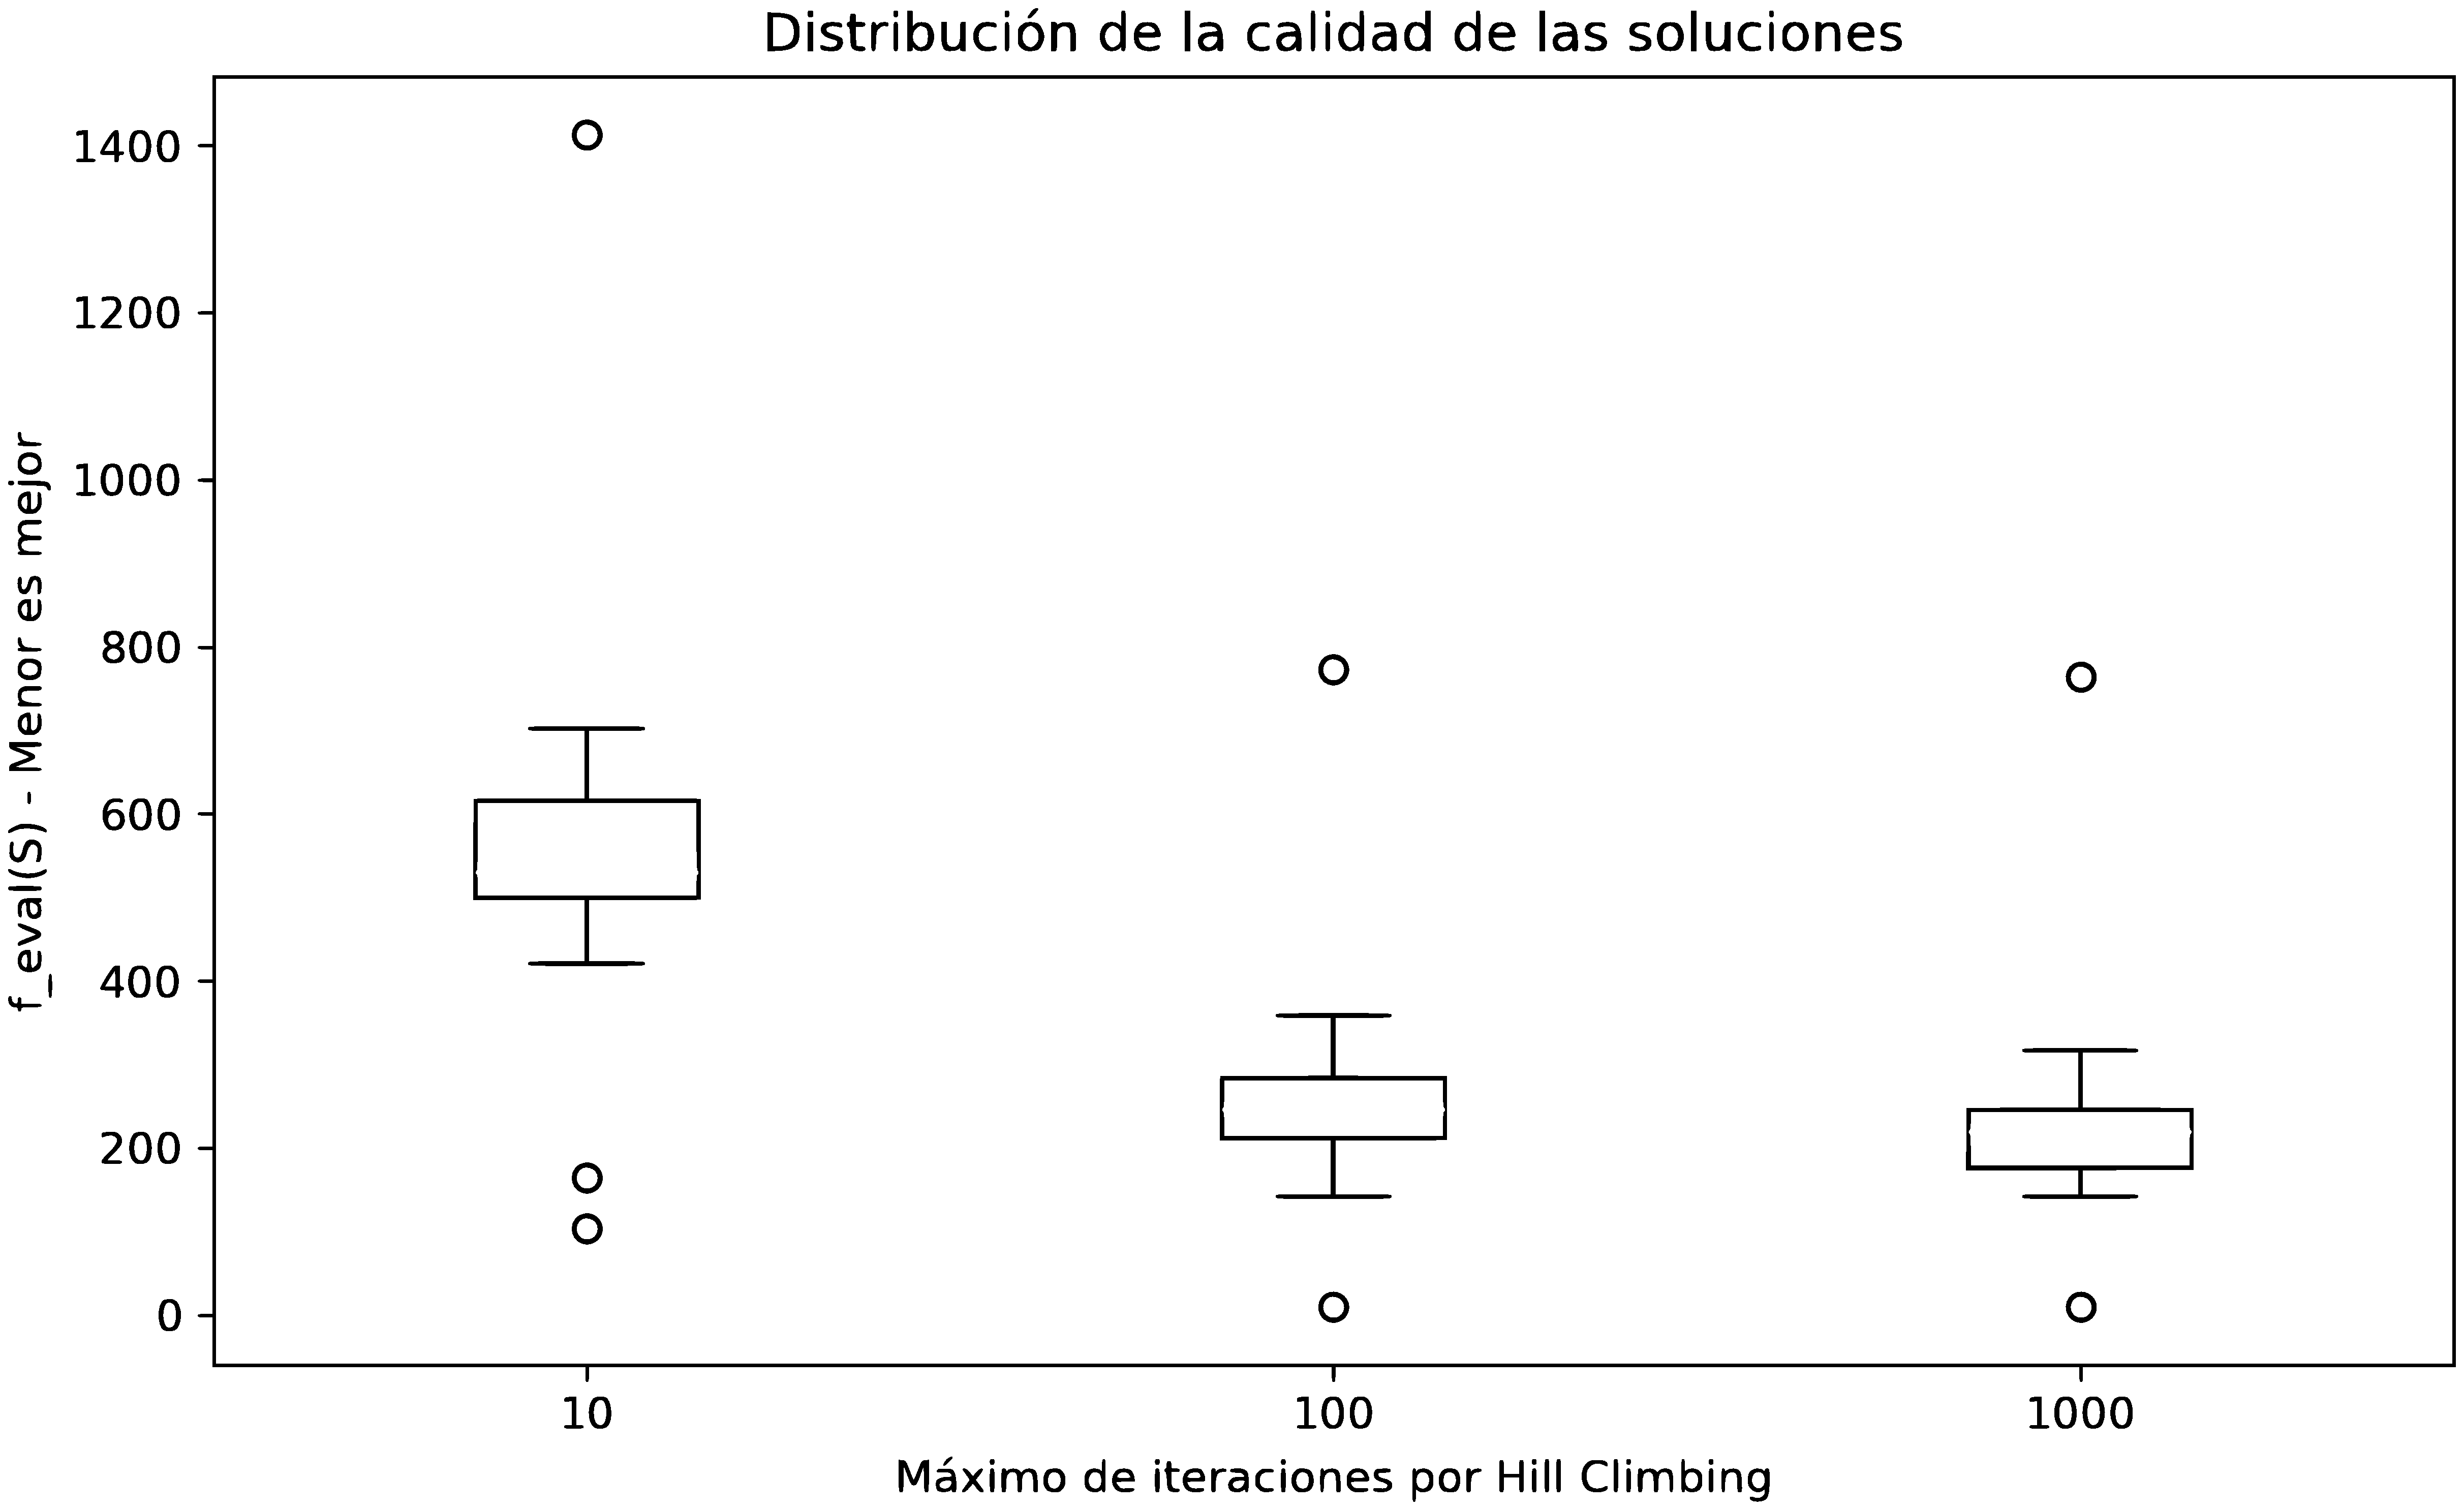
\includegraphics[width=0.6\textwidth]{calidad.eps}
    \caption{ Distribuci\'on calidad de las soluciones}
    \label{fig:mi_imagen}
\end{figure}

Al analizar los resultados de manera individual, se observa que esta mejora fue consistente entre las instancias evaluadas. Al pasar de 10 a 100 iteraciones, las 17 instancias presentaron una disminuci\'on en su penalizaci\'on final. En cambio, al aumentar de 100 a 1000 iteraciones, se obtuvieron mejoras en 14 instancias, mientras que las tres restantes mantuvieron exactamente el mismo resultado. En ning\'un caso se observ\'o un empeoramiento de la soluci\'on. Esto refuerza la idea de que aumentar el l\'imite de iteraciones permite obtener soluciones de mejor calidad, aunque pasadas las 100 iteraciones los beneficios son m\'inimos.

Respecto al tiempo de ejecuci\'on, en la figura 3 se observa un aumento considerable al incrementar el l\'imite de iteraciones de 10 a 100 iteraciones, pero no es igual de importante de 100 a 1000. El promedio pas\'o de 173,25 segundos con 10 iteraciones a 709,97 segundos con 100, lo que representa un incremento promedio del 310\%. En cambio, al pasar de 100 a 1000 iteraciones, el tiempo aument\'o un 20,6\% alcanzando un promedio de 856,37 segundos. Al comparar estos resultados con las mejoras en calidad analizadas previamente, se aprecia que la configuraci\'on de 100 iteraciones ofrece un equilibrio interesante entre calidad y costo computacional, ya que permite obtener gran parte de la mejora observada sin asumir el tiempo adicional que podr\'ia significar la versi\'on con 1000 iteraciones.
\begin{figure}[H]
    \centering
    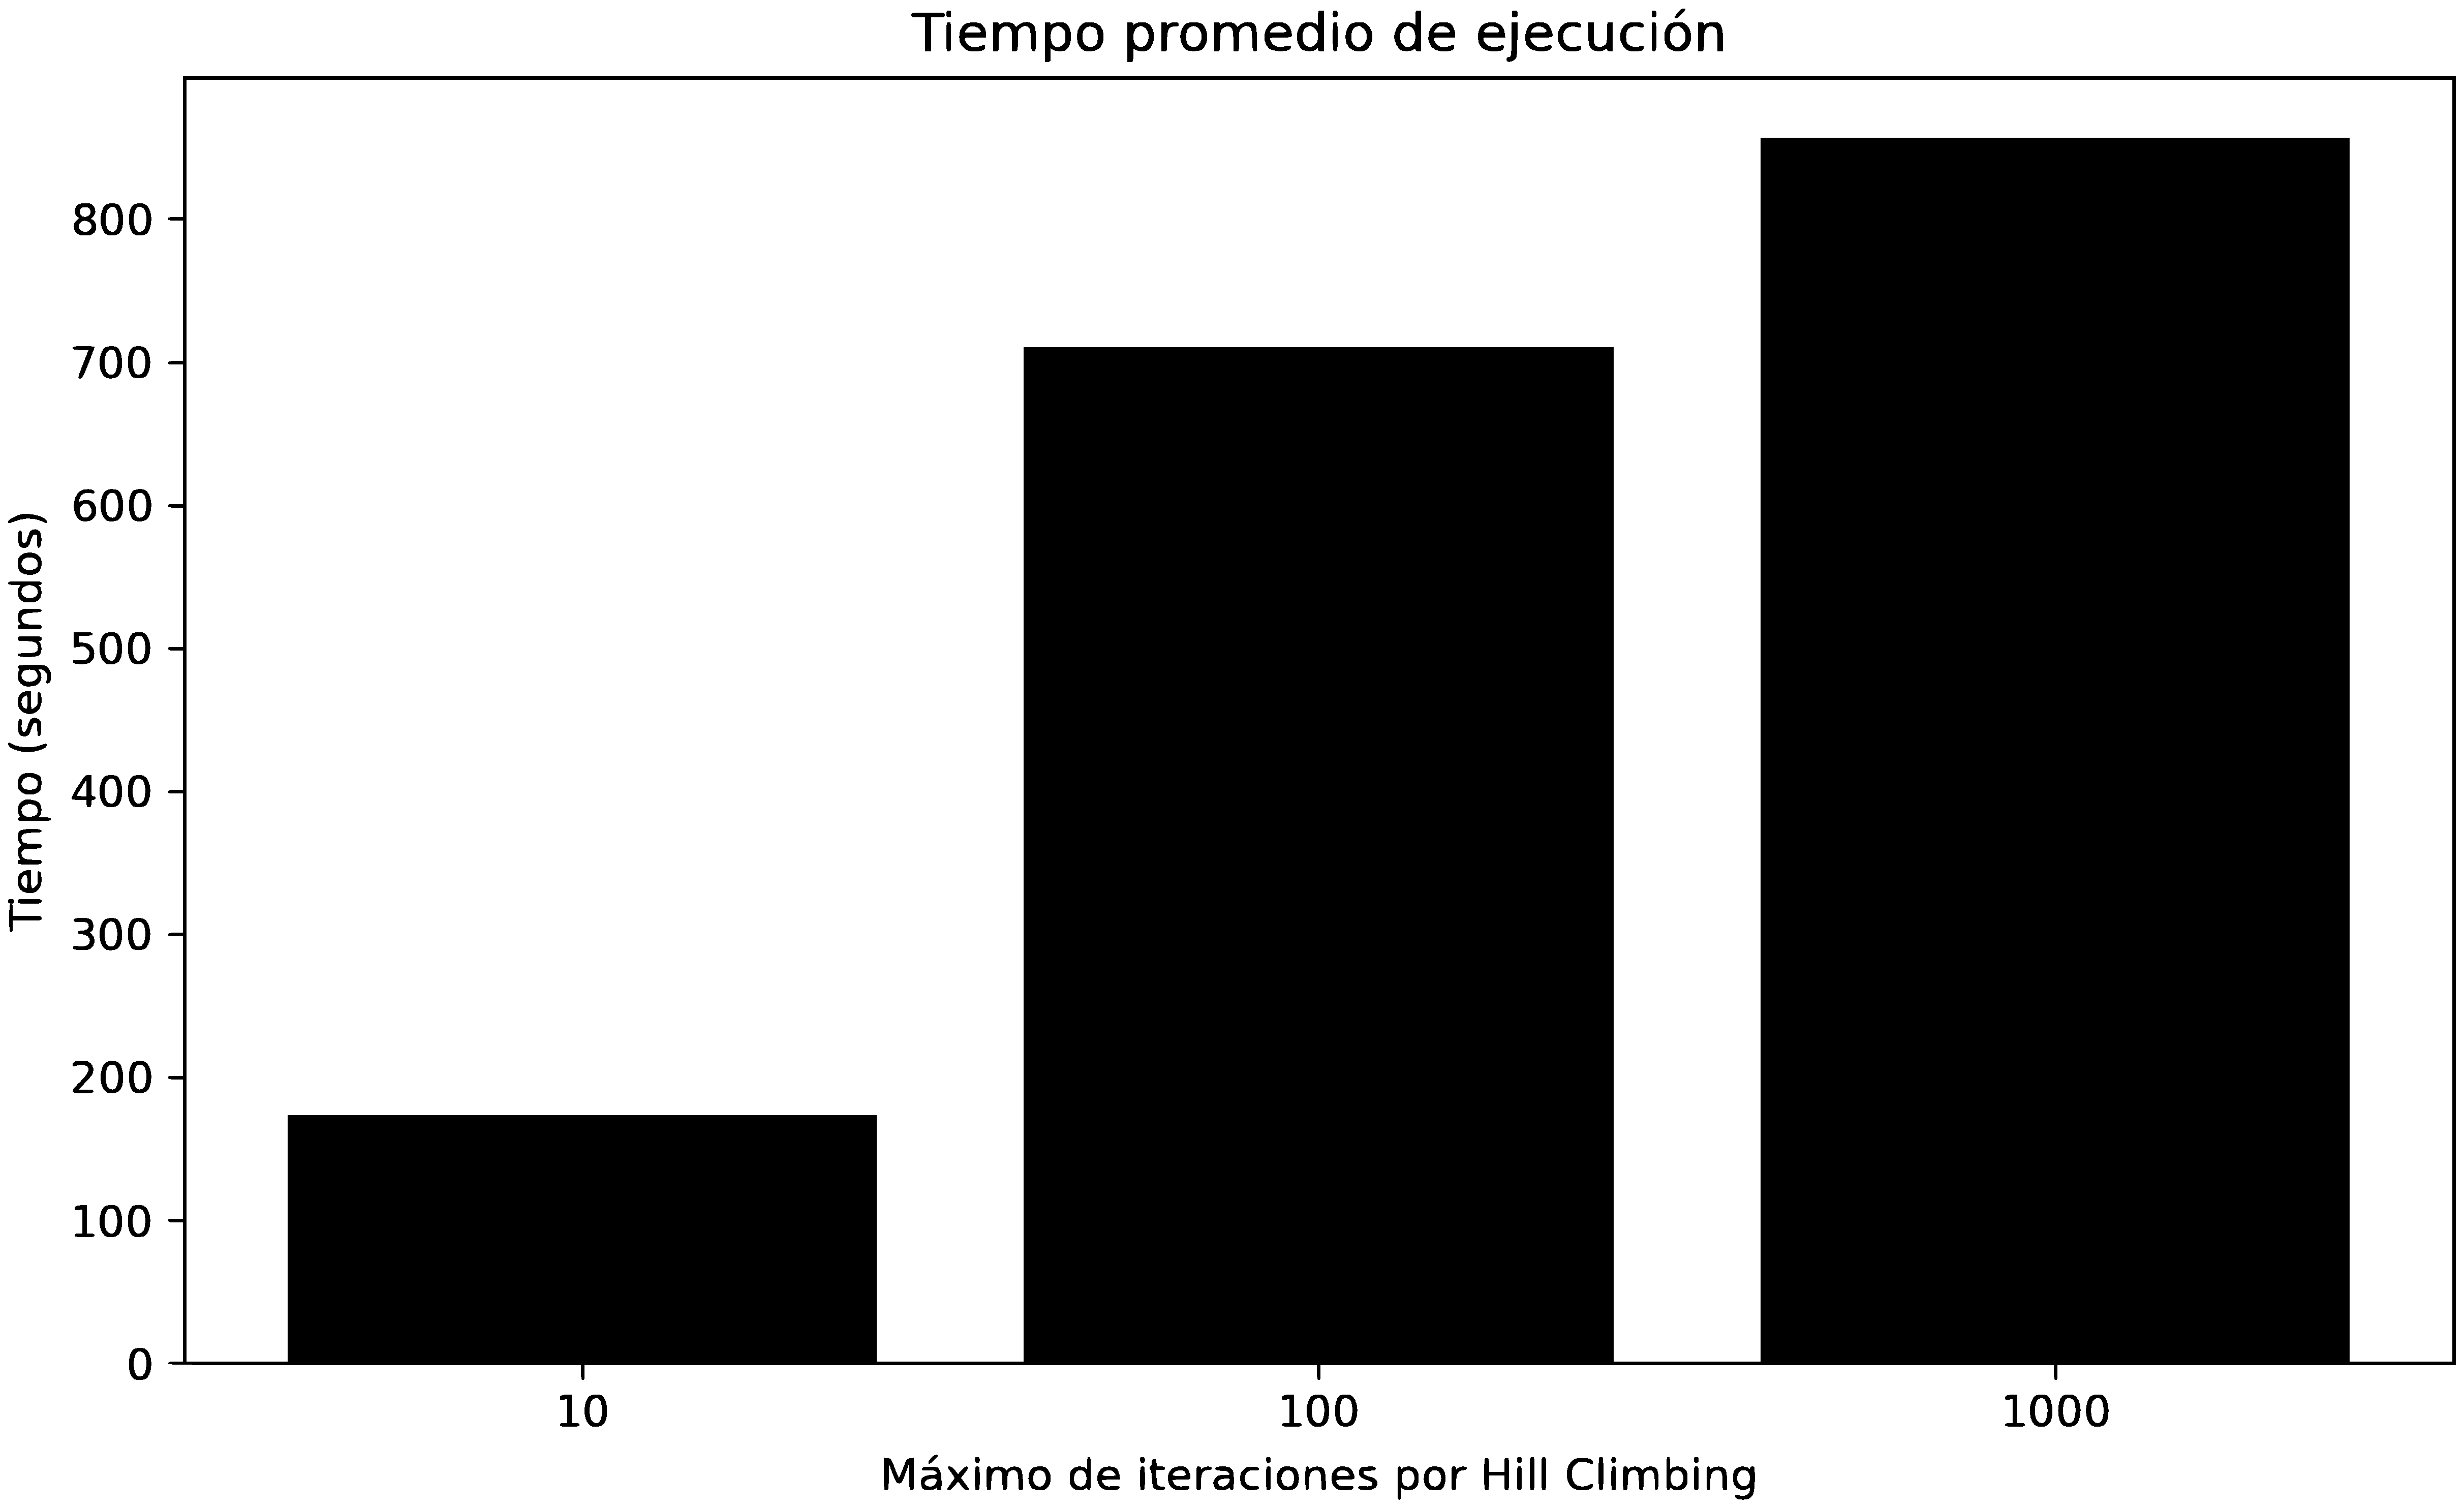
\includegraphics[width=0.6\textwidth]{tiempo_promedio.eps}
    \caption{Tiempo promedio de las ejecuciones}
    \label{fig:mi_imagen}
\end{figure}

En relaci\'on con el comportamiento de la b\'usqueda, se observa que las mejoras m\'as significativas se concentran entre las primeras 100 iteraciones, mientras que el incremento hasta 1000 produce reducciones considerablemente menores en la mejora de la evaluaci\'on. Se considera que esto podr\'ia deberse a que Hill Climbing encuentra inicialmente movimientos que permiten corregir problemas importantes de las soluciones, mientras que, a medida que esta mejora, encontrar movimientos que produzcan reducciones adicionales se vuelve m\'as dif\'icil. Esto podr\'ia indicar que, en una parte importante de las instancias, la b\'usqueda se aproxima a un m\'aximo local alrededor de la 100-\'esima iteraci\'on, haciendo que el algoritmo se detenga antes de llegar m\'as cerca de las 1000.

Esta interpretaci\'on tambi\'en se ve respaldada por el hecho de que tres instancias no presentaron mejoras al pasar de 100 a 1000 iteraciones. Si bien no se dispone del registro expl\'icito del n\'umero de iteraciones efectivamente ejecutadas para confirmar que se haya alcanzado un \'optimo local, los resultados sugieren una tendencia hacia la estabilizaci\'on de las soluciones. En este contexto, aumentar el l\'imite de iteraciones no garantiza mejoras proporcionales, puesto que, llegado al m\'aximo local, el algoritmo no seguir\'a iterando y empezar\'a su l\'ogica de restart.

Un caso particularmente ilustrativo corresponde a la instancia `comp12`, que parti\'o con una funci\'on de evaluaci\'on inicial de 1896. Con 10 iteraciones de Hill Climbing, esta disminuy\'o a 1413, lo que representa una reducci\'on del 25,5\%, con un tiempo de ejecuci\'on de 489,86 segundos. Al aumentar a 100 iteraciones, la evaluaci\'on baj\'o a 773, equivalente a una reducci\'on acumulada del 59,2\% respecto de la soluci\'on inicial y una mejora adicional del 45,3\% respecto del resultado anterior. Sin embargo, este avance implic\'o un aumento del 96\% en el tiempo de ejecuci\'on, alcanzando los 960,19 segundos. Finalmente, con 1000 iteraciones, la penalizaci\'on lleg\'o a 764, lo que supone una mejora adicional de apenas un 1,2\%, mientras que el tiempo aument\'o solo un 2,1\%, hasta los 980,55 segundos. Este caso permite observar c\'omo la mayor parte de la mejora se concentra en las primeras 100 iteraciones, mientras que el aumento posterior del l\'imite produce una reducci\'on mucho m\'as acotada de la evaluaci\'on.

En s\'intesis, los resultados muestran que el algoritmo implementado con Greedy y Hill Climbing con Restart permiti\'o mejorar considerablemente la calidad de las soluciones iniciales en las 17 instancias evaluadas. Sin embargo, estas mejoras no aumentaron proporcionalmente al incrementar el l\'imite de iteraciones, concentr\'andose las mayores diferencias entre las configuraciones de 10 y 100 iteraciones. Si bien utilizar 1000 iteraciones permiti\'o obtener algunas mejoras adicionales, estas fueron m\'as acotadas y requirieron un mayor tiempo de ejecuci\'on. Por lo tanto, considerando conjuntamente la calidad de las soluciones y el costo computacional, la configuraci\'on de 100 iteraciones represent\'o el equilibrio m\'as favorable entre las configuraciones utilizadas.
\section{Conclusiones}
En el presente estudio se analizaron diversas t\'ecnicas que abordan el mismo problema de CB-CTT general, utilizando diferentes perspectivas, tanto en la formulaci\'on como en las estrategias de resoluci\'on. Mientras los m\'etodos exactos buscan obtener resultados \'optimos, los enfoques heur\'isticos y metaheur\'isticos se enfocan en llegar a soluciones sub\'optimas en tiempos razonables. Adem\'as, existen enfoques h\'ibridos y estrategias de selecci\'on de algoritmos que aprovechan las ventajas de diferentes m\'etodos seg\'un la instancia.

Para este experimento, se desarroll\'o un algoritmo de b\'usqueda incompleta basado en una heur\'istica constructiva Greedy, complementada con Hill Climbing con mejor mejora y l\'ogica de Restart. Esta combinaci\'on permiti\'o generar soluciones iniciales, mejorarlas mediante b\'usqueda local y diversificar el proceso para evitar que la b\'usqueda quede limitada a una \'unica soluci\'on.

Los resultados experimentales respaldan los supuestos iniciales de la propuesta, resultando ser una configuraci\'on adecuada para mejorar la calidad de las soluciones iniciales, habiendo logrado mejorar la evaluaci\'on de f\_eval en las 17 instancias y manteniendo el cumplimiento estricto de las Hard Constraints. Sin embargo, la propuesta presenta limitaciones importantes: el algoritmo Greedy no logr\'o construir soluciones iniciales para cuatro instancias, mientras que la b\'usqueda local se restringi\'o a los movimientos Time Move y Room Move, descartando Lecture Move por su elevado costo computacional. Adem\'as, los resultados muestran que aumentar el l\'imite de iteraciones de 100 a 1000 produce mejoras relativamente peque\~nas frente al tiempo adicional requerido.

Como trabajo futuro, resultar\'ia relevante mejorar la heur\'istica constructiva del algoritmo Greedy, para aumentar la tasa de generaci\'on de soluciones iniciales, as\'i como incorporar nuevos movimientos que permitan explorar regiones del espacio de soluciones que actualmente no son alcanzadas. Finalmente, tambi\'en ser\'ia interesante repetir el experimento, pero almacenando otros datos adicionales, como el n\'umero de iteraciones por repetici\'on del algoritmo o los valores de evaluaci\'on de todas las soluciones entregadas por Greedy.

\section{Uso LLMs}
\begin{enumerate}
\item Herramienta utilizada: ChatGPT modelo GPT-5.6 Luna plan Go
\item Prop\'osito de uso: Revisar redacci\'on, explicar modelos, traspasar a LaTex, depurar c\'odigo, debuggear y ayudar con implementaciones puntuales
\item Prompts relevantes: "Revisa la redacci\'on en este parrafo, para que se encuentre en tercera persona". "Traspasa estas variables a LaTex". "Tengo este strcuct, con X m\'etodo. ¿Sabes decirme d\'onde est\'a el error?"
\item Nivel de edici\'on: Las correcciones propuestas a lo escrito originalmente se revisaron y algunas fueron aplicadas y otras no seg\'un diversos criterios. Los traspasos a LaTex fueron princpalmente copiados y pegados, pues correspond\'ian directamente a lo previamente escrito a mano en el texto original. Las depuraciones de c\'odigo fueron evaluadas ley\'endolas y ejecutando ciertas parte de c\'odigo, se modifi\'o el original cuando la ayuda s\'i funcionaba.
\item Validaci\'on: Juicio propio, Papers utilizados en la bibliograf\'ia.
\end{enumerate}


\bibliographystyle{plain}
\bibliography{Referencias}

\end{document} 
